\documentclass[a4paper, titlepage]{report}

\usepackage[francais]{babel}
\usepackage[utf8]{inputenc}
\usepackage[T1]{fontenc}

\usepackage{listings}
\usepackage{titlesec}
\usepackage{color}
\usepackage{graphicx}

\titleformat{\chapter}[display]
  {\bfseries\Large}
  {\filright\textsc{\chaptertitlename} \LARGE\thechapter}
  {1ex}
  {\titlerule\vspace{1ex}\filleft}
  [\vspace{1ex}\titlerule]


\definecolor{gris}{rgb}{0.97,0.97,0.97}
\definecolor{vert}{rgb}{0,0.6,0}
\definecolor{mauve}{rgb}{0.5,0,0.5}
\definecolor{rose}{rgb}{1,0.5,1}
\definecolor{cyan}{rgb}{0.1,0.4,0.6}
\definecolor{marron}{rgb}{0.4,0.2,0}
\definecolor{jaune}{rgb}{1,0.6,0}
\definecolor{bleu}{rgb}{0,0,0.8}

\lstset{
	language=R,	
	frame=tblr,
	numbers=left,
	breaklines=true,
	backgroundcolor=\color{gris},
    basicstyle=\small\ttfamily,
    stringstyle=\color{vert},
    otherkeywords={0,1,2,3,4,5,6,7,8,9},
    morekeywords={TRUE,FALSE},
    deletekeywords={data,frame,length,as,character},
    keywordstyle=\color{blue},
    commentstyle=\color{vert},
}


\title{Rapport Projet SY09}
\date{3 mai 2018}
\author{Yiqing \textsc{Su} et Théophile \textsc{Molcard}}


\begin{document}

\renewcommand{\chaptername}{Partie}


\maketitle

\tableofcontents



\chapter{Cuisine}

Le jeu de données à étudier de la première partie est un ensemble de recettes de cuisine de diverses origines.\\
\indent Pour la question de 1.1 jusqu'à 1.5, le jeu de données utilisé est une version agrégée par origine. Puis pour les restes questions, il s'agit d'utiliser les données sans agrégation, autrement dit, il y a toutes les recettes de chaque pays ou région.

\section{Analyse exploratoire}
Le premier jeu de données comporte 26 lignes et 51 colonnes. Une ligne représente une information synthétique d'une recette pour un pays ou une région. Puis la première colonne indique le nom du pays ou de la région et les autres colonnes représentent l'utilisation des 50 ingrédients dans la recette.\\
\indent Avec \textbf{boxplot} et \textbf{summary}, nous pouvons voir que les données sont toutes entre 0 et 1. La moyenne pour chaque boîte à moustache est inférieur à 0,5. Plus que deux tiers des pays ou des régions choisis ne sont pas asiatiques. Donc, certains ingrédients comme "olive oil" et "cayenne" ont plus de variances parce que une partie de recettes utilisent beaucoup cet ingrédient et les autres non. Certains ingrédients comme "soy sauce" et "sesame oil" sont faibles à la moyenne et à la variance parce que seulement les pays et les régions asiatiques vont les utiliser.
\indent Nous nous intéressons par la corrélation entre les données. Pour les ingrédients, 

\section{Analyse en composantes principales}
La matrice que l'on étudie est de dimension $M_{26,50}$, elle est donc de rang inférieur à 26. L'inertie peut donc être entièrement expliquée par 26 composantes. En effectuant une ACP sur ces données on obtient donc les 26 composantes principales expliquant l'inertie du nuage de points. Si l'on cherche les valeurs propres de la matrice de covariance, on constate comme attendu que 24 des valeurs propres qui résultent sont nulles.\\

\newpage
On peut donc afficher l'inertie expliquée par chaque composantes et par la somme des n premiers axes.
\begin{figure}[h]
	\begin{center}
		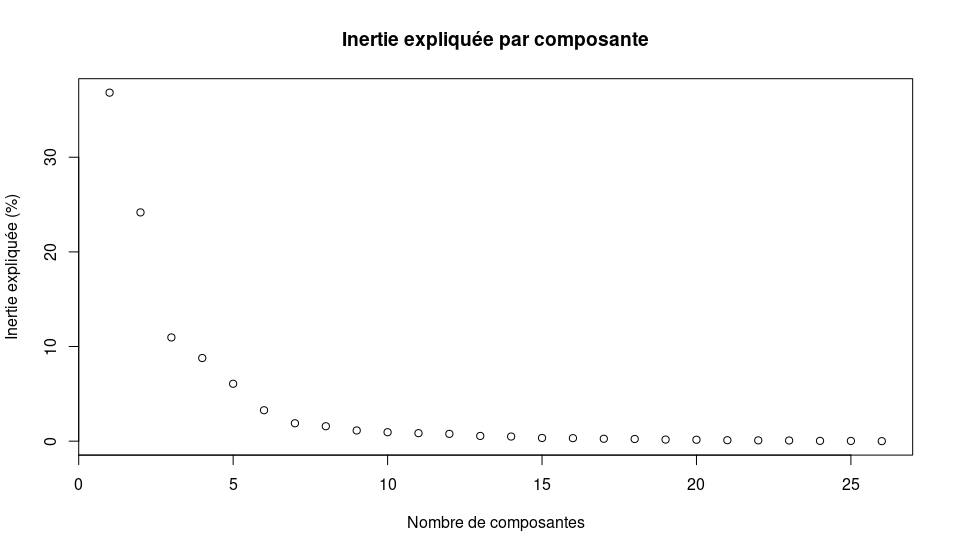
\includegraphics[scale = 0.32]{./doc/plot-inertie-par-composantes.png}
		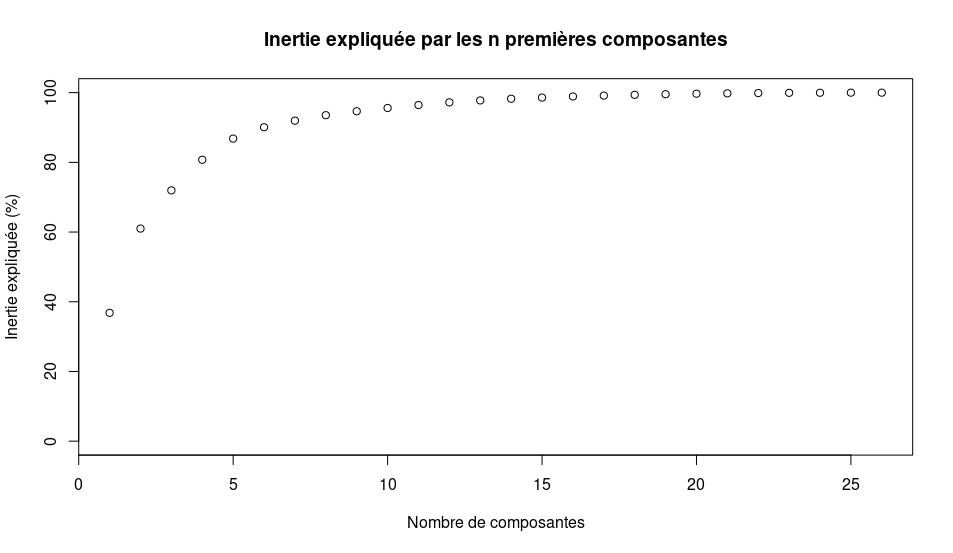
\includegraphics[scale = 0.32]{./doc/plot-inertie-n-composantes.png}
	\end{center}
\end{figure}

On constate que les deux premières composantes, bien qu'insuffisantes pour expliquer complètement les différences entre tous les points, permettent d'expliquer plus de 60\% de l'inertie. Il peut donc être intéressant d'afficher les points en fonction de ces composantes.
\begin{figure}[h]
	\begin{center}
		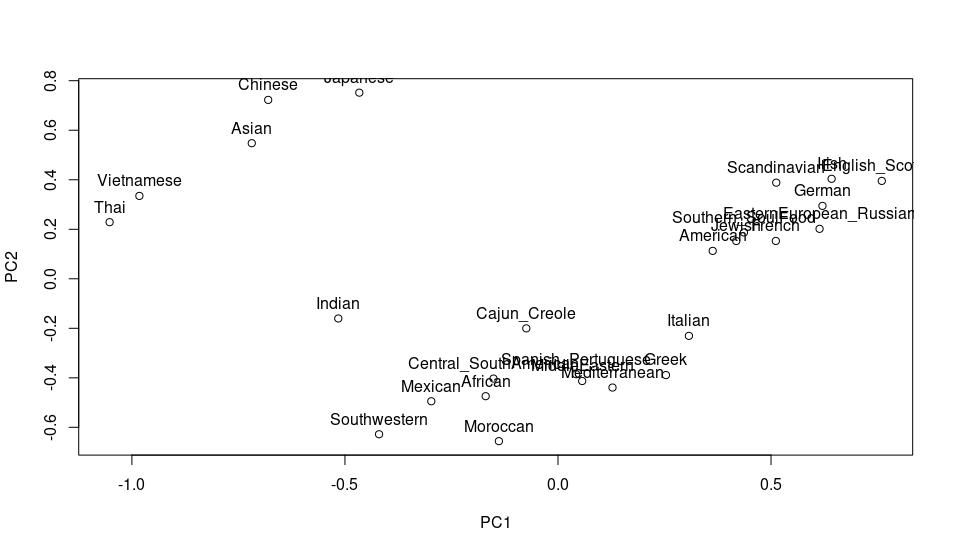
\includegraphics[scale = 0.32]{./doc/plot-recettes-composantes-1-2.png}
	\end{center}
\end{figure}

Par ce simple graphique on constate déjà certains regroupement entre les recettes des différents pays, avec trois groupes principaux qui ressortent. grossièrement on a les recettes des pays asiatiques, des pays occidentaux et des pays méditerranéens. Ces deux composantes sont cependant insuffisantes à expliquer l'ensemble des subtilités de ces données, 6 composantes sont nécessaire pour expliquer 90\% de l'inertie.


\section{Analyse ascendante hiérarchique}

\section{K-Means}

\section{Comparaison}

\section{Analyse descriptive}

\section{Similarité - Dissimilarité}

\section{Classification ascendante hiérarchique}

\section{K-Médïodes}



\chapter{K-Means Adaptatif}


\section{Données synthétiques}

\section{Iris}

\section{Spam}



\chapter*{Annexe}
\lstinputlisting[firstline=0, lastline=108]{./doc/partie-1.R}


\end{document}